\section{Functionality}
In this section, we describe the main features and functionality of the Safety Annex. 

\subsection{Nominal Model}
An AADL model of the nominal system behavior includes mechanical and digital components and their interconnections. This nominal model is then annotated with assume-guarantee contracts using the AGREE annex for AADL ~\cite{NFM2012:CoGaMiWhLaLu}. Using compositional verification techniques, the nominal model behavior can be seen in the absence of faults. 

\subsection{Fault Model}
Once the nominal model behavior is defined and verified, the Safety Annex can be used on each of the system components that may be affected by faults. The faults are defined on each of the relevant components using a predefined customizable library of fault nodes. This extended model is then analyzed and the behavior of the system in the presence of faults can be seen. Separation of the nominal model from the fault model is handled through a selection mechanism provided to the user. The nominal model behavior can be defined and verified without also running safety analysis. 

\subsection{Grammar and Syntax}
To illustrate the grammar and syntax of the Safety Annex, we will use an example from the Wheel Brake System described in ~\cite{AIR6110} and used in our previous work ~\cite{Stewart17:IMBSA}. 

The fault library contains commonly used fault node definitions. An example of a fault node is shown in Figure~\ref{fig:faultNodeDef}. The \textit{fail\_to} node provides a way to input a failure value and if the fault is triggered, then the nominal component output value is overridden by the \textit{fail\_to} failure value. 

%%%%%%%%%%%%%%% fail_to fault node definition figure here
\begin{figure}
\begin{center}
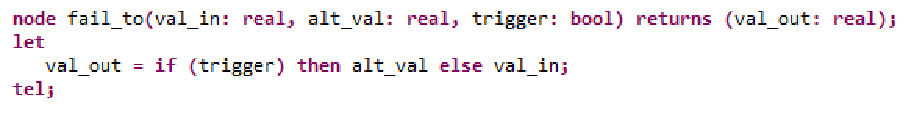
\includegraphics[width=1.0\textwidth]{images/faultNode.png}
\end{center}
\vspace{-0.2in}
\caption{Fault Node Definition}
\label{fig:faultNodeDef}
\end{figure}

In the WBS, the Selector valve component receives inputs from the hydraulic pressure pumps and a digital system component. The Selector will change modes of the system depending on the inputs it receives (see ~\cite{AIR6110,Stewart17:IMBSA} for more information). There are two main hydraulic lines that feed into the Selector, namely the green line (normal mode of operation) and the blue line (alternate mode). The output of the Selector component will either be the green or the blue hydraulic fluid. To motivate the description of the syntax, we will go through a fault on the Selector component that describes a nondeterministic value output on the blue hydraulic line as shown in Figure ~\ref{fig:annex}. \\

%%%%%%%%%%%%%%% safety annex figure here
\begin{figure}
\begin{center}
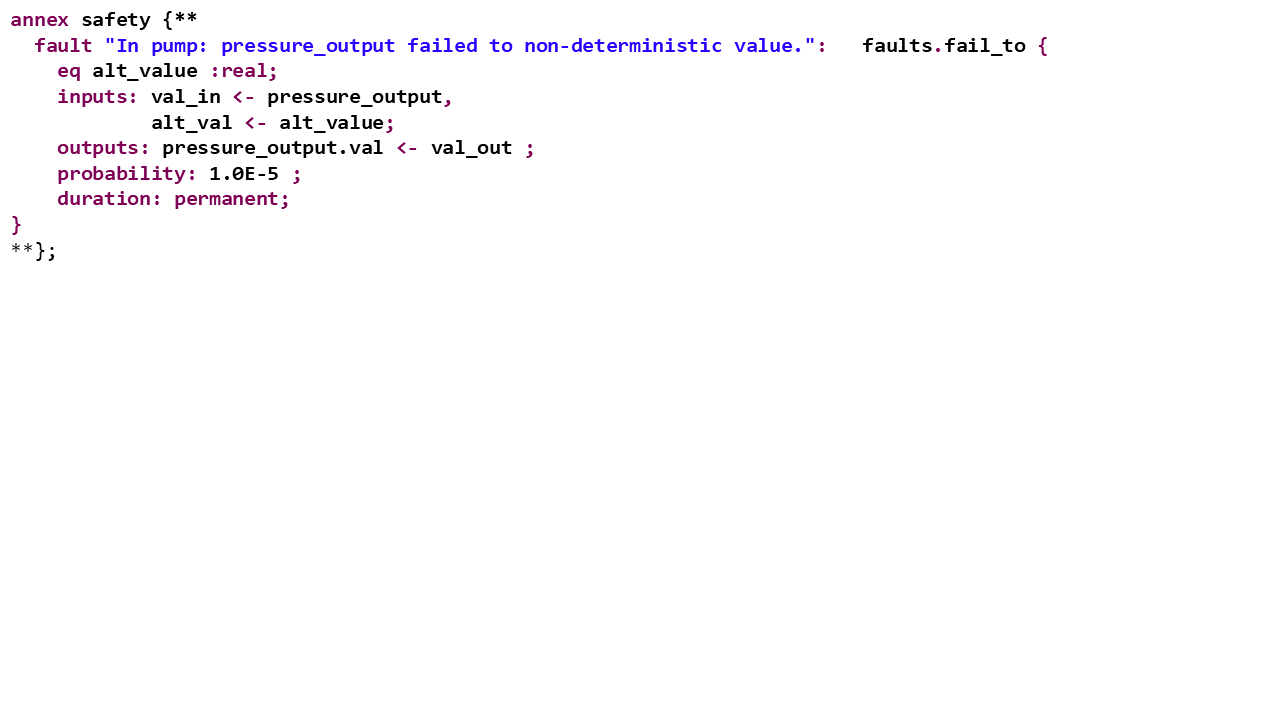
\includegraphics[width=1.0\textwidth]{images/annex.png}
\end{center}
\vspace{-0.2in}
\caption{Safety Annex Fault Definition}
\label{fig:annex}
\end{figure}

The \textit{fault statement} consists of a unique description string, the fault node definition name, and a series of \textit{fault subcomponent} statements. \\

\textbf{Inputs}: The inputs in a fault statement are the parameters into the fault node definition. As shown in Figure~\ref{fig:annex}, \textit{val\_in} and \textit{alt\_val} are the two parameters into the fault node. These are linked to the values found in \textit{blue\_output.val}, the output from the Selector component, and \textit{alt\_value}, a nondeterministic value defined within the Safety Annex. When the analysis is run, these values are passed into the fault node definition. 

\textbf{Outputs}: The outputs of the fault definition correspond to the outputs of the fault node. The fault output statement links the component output (\textit{blue\_output.val}) with the fault node output (\textit{val\_out}). If the fault is triggered, the nominal value of \textit{blue\_output.val} is overridden by the failure value output by the fault node \textit{val\_out}.

\textbf{Duration}: The duration of the fault in this example is permanent. 

\textbf{Equation Statements}: Equation statements support deterministic or nondeterministic types. An example of nondeterministic equation statement is shown in Figure~\ref{fig:annex}. For more details on equation statements, see ~\cite{NFM2012:CoGaMiWhLaLu}.\\





